\documentclass{article} % For LaTeX2e
\usepackage{nips15submit_e,times}
\usepackage{hyperref}
\usepackage{url}
%\documentstyle[nips14submit_09,times,art10]{article} % For LaTeX 2.09
\usepackage{amsmath}
\usepackage{graphicx}
\usepackage{subfig}
\title{Report}


\author{
David S.~Hippocampus\thanks{ Use footnote for providing further information
about author (webpage, alternative address)---\emph{not} for acknowledging
funding agencies.} \\
Department of Computer Science\\
Cranberry-Lemon University\\
Pittsburgh, PA 15213 \\
\texttt{hippo@cs.cranberry-lemon.edu} \\
\And
Coauthor \\
Affiliation \\
Address \\
\texttt{email} \\
\AND
Coauthor \\
Affiliation \\
Address \\
\texttt{email} \\
\And
Coauthor \\
Affiliation \\
Address \\
\texttt{email} \\
\And
Coauthor \\
Affiliation \\
Address \\
\texttt{email} \\
(if needed)\\
}

% The \author macro works with any number of authors. There are two commands
% used to separate the names and addresses of multiple authors: \And and \AND.
%
% Using \And between authors leaves it to \LaTeX{} to determine where to break
% the lines. Using \AND forces a linebreak at that point. So, if \LaTeX{}
% puts 3 of 4 authors names on the first line, and the last on the second
% line, try using \AND instead of \And before the third author name.

\newcommand{\fix}{\marginpar{FIX}}
\newcommand{\new}{\marginpar{NEW}}

%\nipsfinalcopy % Uncomment for camera-ready version

\begin{document}
\maketitle

\section{Softmax Regression via Gradient Descent}
\subsection{Problem definition}
In this problem, we need to classify MNIST datasets using softmax regression. In the experiments, we only use the first 20,000 training images and the last 2,000 test images.

\subsection{Methods}
\textbf{Derive the gradient for Softmax Regression:} \\
The cross-entropy cost function can be expressed as,

\begin{equation}
	E = - \sum_{n}\sum_{k=1}^{c}t_k^n\ln y_k^n
\end{equation}

Where, 
\begin{equation}
	y_k^n = \frac{\exp{(a_k^n)}}{ \sum_{k'}\exp{(a_{k'}^n})}
\end{equation}
And, 
\begin{equation}
	a_k^n = w_k^Tx^n
\end{equation}
We can calculate the gradient for softmax regression as follows,
\begin{equation}
\begin{split}
-\frac{\partial E^n(w)}{\partial w_{jk}}& = - \frac{\partial E^n(w)}{\partial a_k^n}\frac{\partial a_k^n}{\partial w_{jk}} \\
& = -\sum_{k'} \frac{\partial E^n(w)}{\partial y^n_{k'}} \frac{\partial y^n_{k'}}{\partial a^n_k}\frac{\partial a_k^n}{\partial w_{jk}} \\
\end{split}
\end{equation}
And 
\begin{equation}
\begin{split}
\frac{\partial y^n_{k'}}{\partial a^n_k} =  y^n_{k'}\delta_{kk'} - y_{k
'}y_{k}\\
\end{split}
\end{equation}
Where $\delta_{kk} = 1$ if $k = k'$, otherwise $\delta_{kk} = 0$.
And
\begin{equation}
\begin{split}
	\frac{\partial E^n(w)}{\partial y^n_{k'}} = -\frac{t_{k'}}{y_{k'}}
\end{split}
\end{equation}
Substitute Equation (5) and Equation (6) into Equation (4) we get,
\begin{equation}
\begin{split}
	-\frac{\partial E^n(w)}{\partial w_{jk}} = (t_k - y_k)x_j^n 
\end{split}
\end{equation}


\textbf{Preprossing}: First, we extract the first 20,000 training images and the last 2,000 test images. Then normailize the images to make sure the pixel values are in the range of [0,1]. Convert the labels to one-hot vectors. Divide the training images into two parts, the first 10\% are used for as a hold-out set and the rest 90\% are used for training.
\\
\textbf{Experiments settings:}We use an initial learning rate $\eta({0})$ = 0.004 and use equation $\eta({t}) = \eta{(0)}/(1+t/T)$ to anneal the learning rate by reducing it over time. $t$ is used to index the epoch number and $T$ is a metaparameter which is set to be 2. In the
experiements, we find that above learning settings work best.   \\
To determine the best type of regurization and the best $\lambda$, we try $L_2$ regularization and $L_1$ regularization seperately. For the $L_2$ regularizartion, we search the best $\lambda$ in the set $\{0.01, 0.001, 0.0001\}$. If the accuracy on the hold-out set decreases for 3 epochs, we stop the algorithm and use the weights with the highest accuracy on the hold-out set as the final answer. For the $L_1$ regularization, we follow the same steps. We run the 1000 epochs for each setting. \textbf{}Then we compare the results got from these two regularization methods and use the best one as the final result.
 
\subsection{Results}
(a) In the experiments, we find that using $L_2$ regularization with $\lambda = 0.01$ obtain the best result on the validation set with an accuracy of 0.9045\% on the validation set. The accuracy is 0.927\% on the test set under such settings. \\

To further examine the performance of the algorithm, we try other $\lambda$s. We choose $\lambda$ in the set $\{0.05,0.005,0.0005\}$ and use $L_2$ regularization. The highest accuracy on the validation set is $0.8965\%$ with $\lambda = 0.0005$. And the test accuracy is $0.933\%$ which is slightly higher than when $\lambda = 0.01$. So in following experiments, we fix $\lambda$ to be 0.0005.

\begin{figure}%
	\centering
	\subfloat[The percent correct over the number of training iterations for the training, hold-out and test set.]{{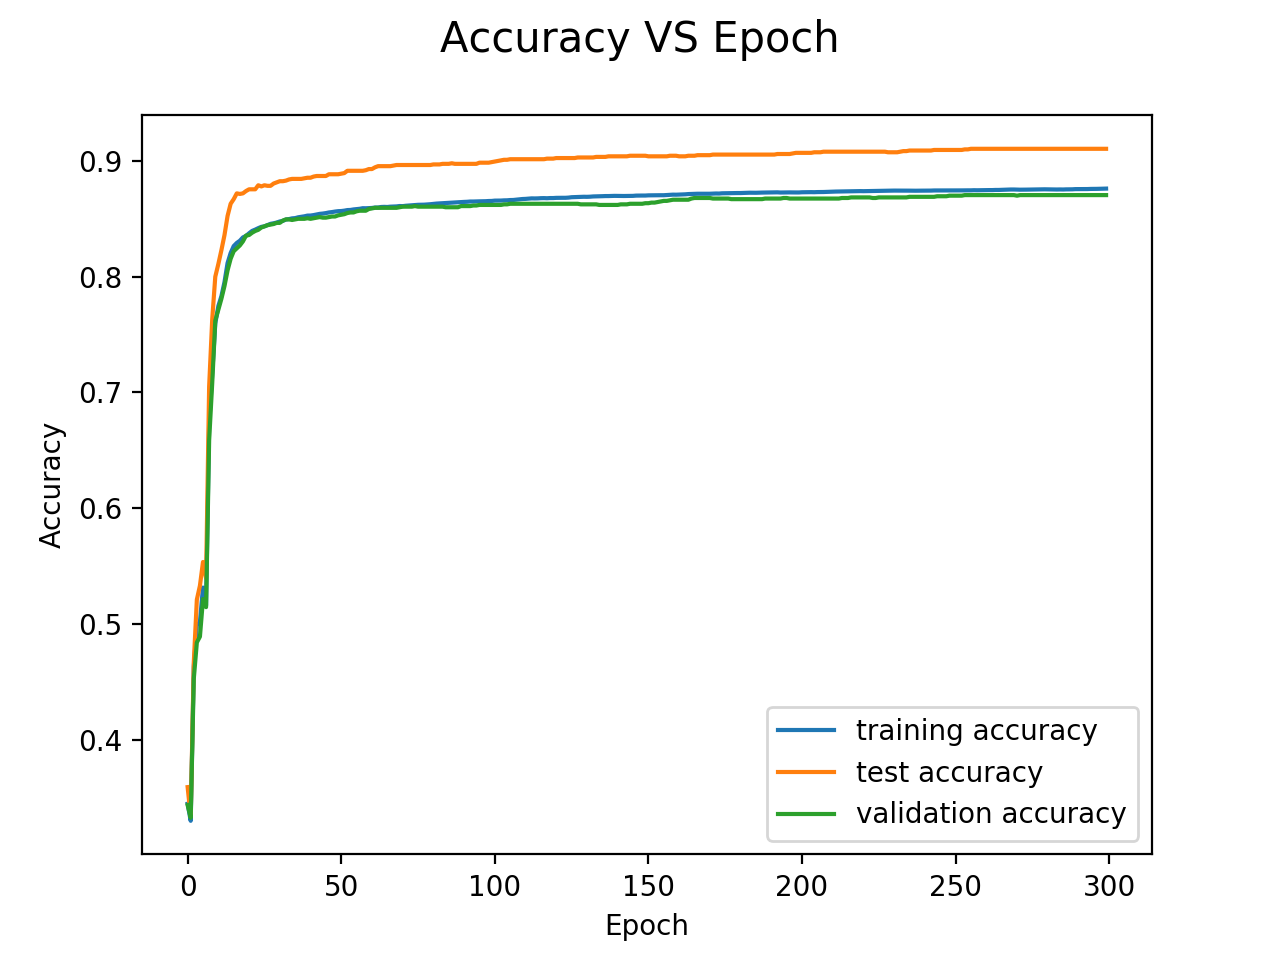
\includegraphics[width=1.8in,height=1.8in]{../softmax/figs/accuracy.png} }
		\label{fig: 1}
	}%
	\qquad
	\subfloat[The value of the loss function over the number of training iterations for the training, hold-out, and test set.]{{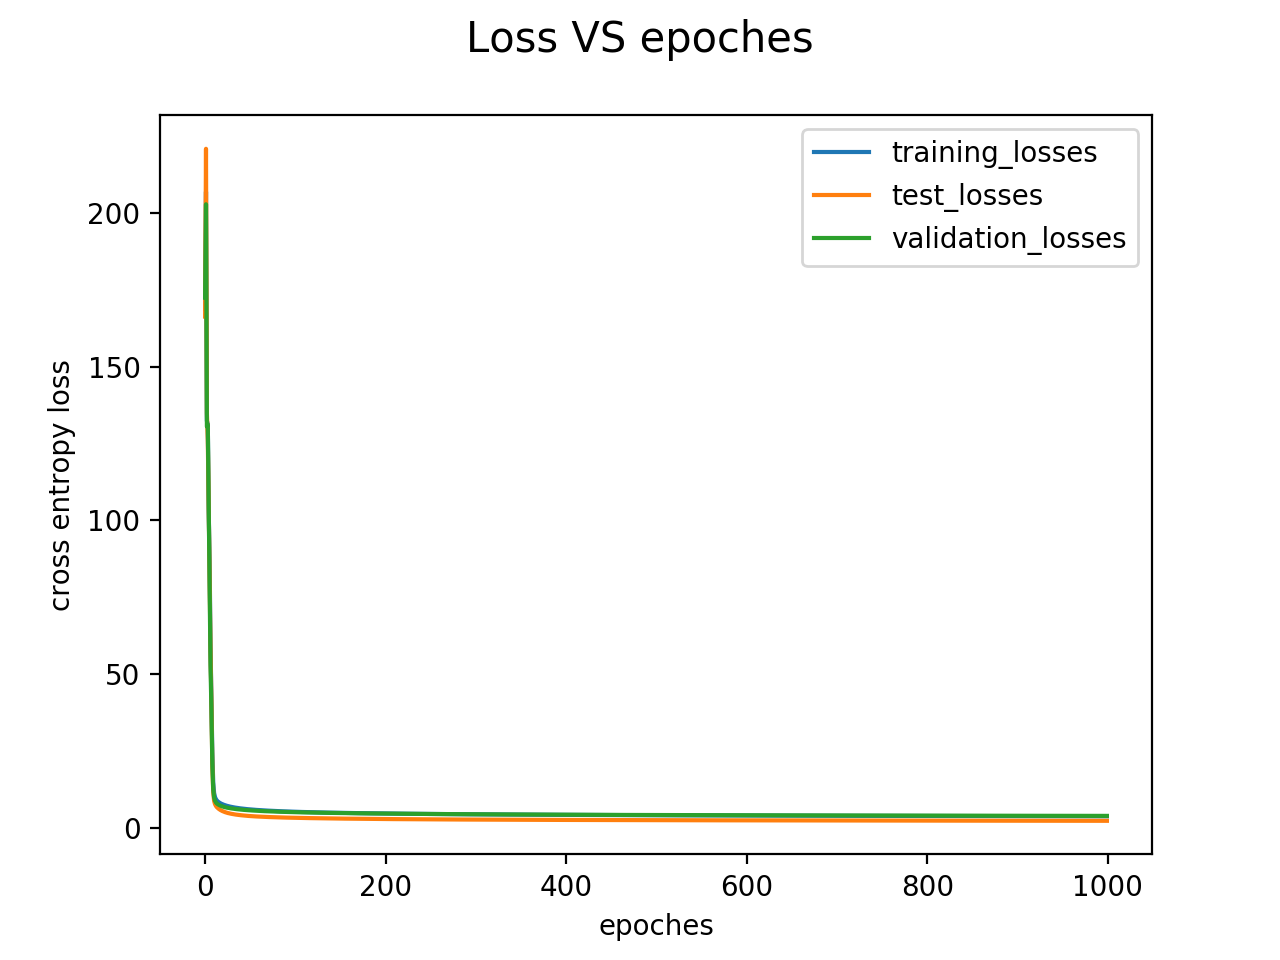
\includegraphics[width=1.8in,height=1.8in]{../softmax/figs/loss.png}  }
			\label{fig: 2}%
		}%
	\caption{The performance of the algorithm over the number of training iterations. }%
\end{figure}



(b) In this experiement, we use $L_2$ regularization with $\lambda = 0.005$. The figure is shown in Fig \ref{fig: 1}.


(c) In this experiement, we use $L_2$ regularization with $\lambda = 0.005$. The figure is shown in Fig \ref{fig: 2}.

(d) We plot the results in Fig \ref{figure: 3}. We can see that the image of the weight and the corresponding image of the average digit is almost the same. The reason is that we classify the images based on the inner product of the pixesls with the weights. And the inner product is maximized when the angle between the weight and the image is zero. So we see that the image of the weight and the corresponding image of the average digit is similar.

\begin{figure}[h]
	\centering	
	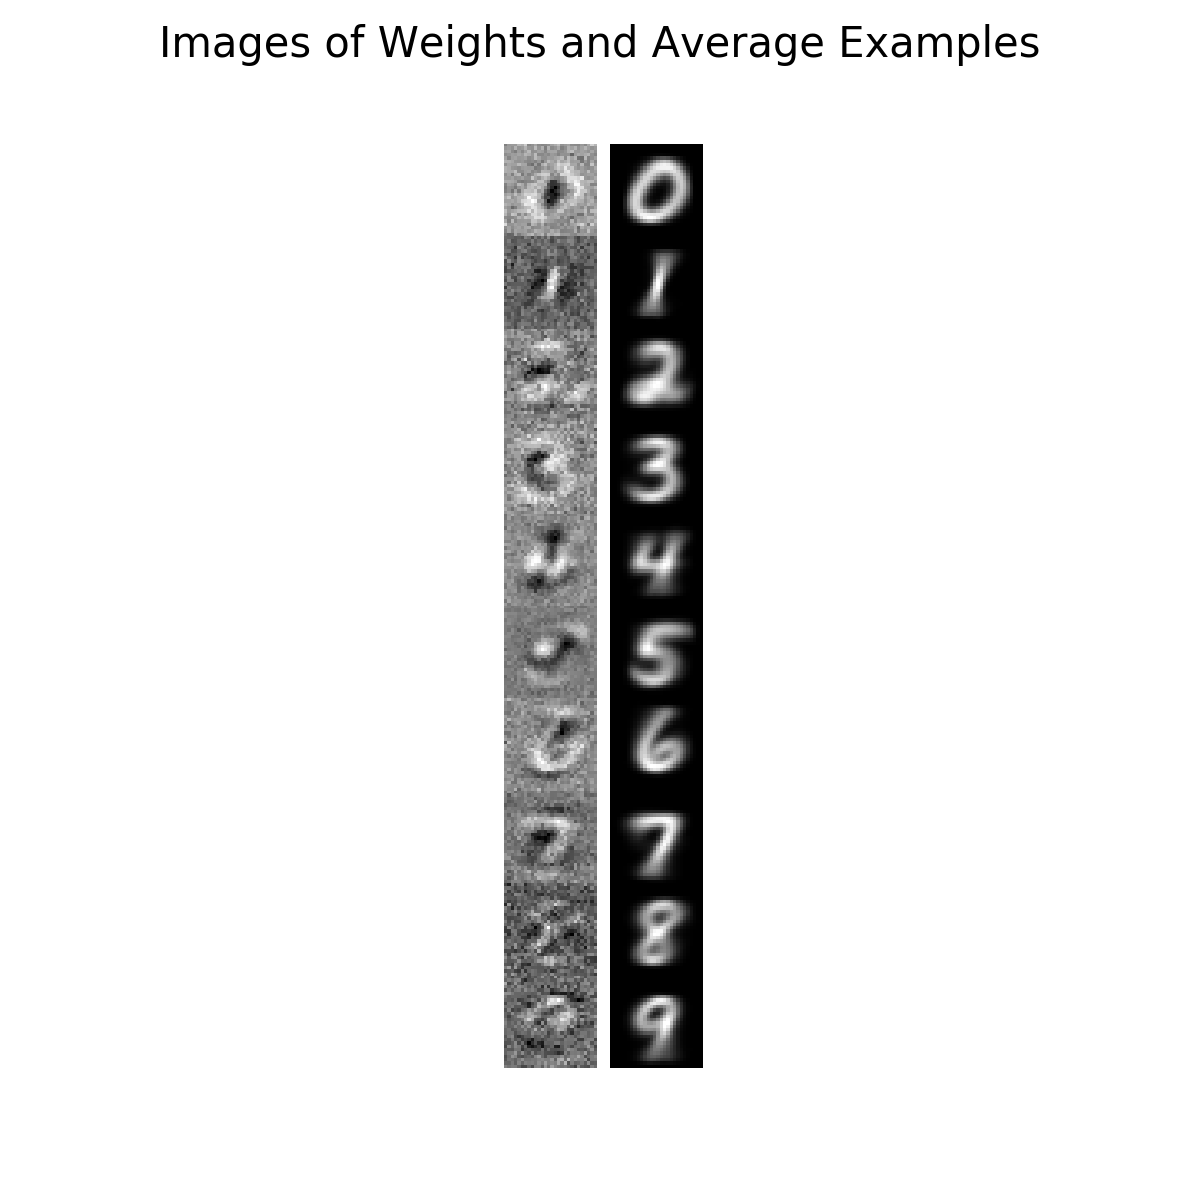
\includegraphics[width=2.8in,height=3.2in]{../softmax/figs/image_of_weights_and_digits.png} 
	\caption{}
	\label{figure: 3}
\end{figure}

\subsection{Discussion}




\subsubsection*{Acknowledgments}

. 

\subsubsection*{References}

\end{document}